\documentclass[a4paper]{article}

\usepackage[pages=all, color=black, position={current page.south}, placement=bottom, scale=1, opacity=1, vshift=5mm]{background}
\usepackage[margin=1in]{geometry} % full-width

% AMS Packages
\usepackage{amsmath}
\usepackage{amsthm}
\usepackage{amssymb}
\usepackage{multirow}
\usepackage{adjustbox} 

% Unicode
\usepackage[utf8]{inputenc}
\usepackage{hyperref}
\hypersetup{
	unicode,
%	colorlinks,
%	breaklinks,
%	urlcolor=cyan, 
%	linkcolor=blue, 
	pdfauthor={Author One, Author Two, Author Three},
	pdftitle={A simple article template},
	pdfsubject={A simple article template},
	pdfkeywords={article, template, simple},
	pdfproducer={LaTeX},
	pdfcreator={pdflatex}
}

% Vietnamese
%\usepackage{vntex}

% Natbib
\usepackage[sort&compress,numbers,square]{natbib}
% \bibliographystyle{mplainnat}
\bibliographystyle{plainnat}

% Theorem, Lemma, etc
\theoremstyle{plain}
\newtheorem{theorem}{Theorem}
\newtheorem{corollary}[theorem]{Corollary}
\newtheorem{lemma}[theorem]{Lemma}
\newtheorem{claim}{Claim}[theorem]
\newtheorem{axiom}[theorem]{Axiom}
\newtheorem{conjecture}[theorem]{Conjecture}
\newtheorem{fact}[theorem]{Fact}
\newtheorem{hypothesis}[theorem]{Hypothesis}
\newtheorem{assumption}[theorem]{Assumption}
\newtheorem{proposition}[theorem]{Proposition}
\newtheorem{criterion}[theorem]{Criterion}
\theoremstyle{definition}
\newtheorem{definition}[theorem]{Definition}
\newtheorem{example}[theorem]{Example}
\newtheorem{remark}[theorem]{Remark}
\newtheorem{problem}[theorem]{Problem}
\newtheorem{principle}[theorem]{Principle}

\usepackage{graphicx, color}
\graphicspath{{fig/}}

%\usepackage[linesnumbered,ruled,vlined,commentsnumbered]{algorithm2e} % use algorithm2e for typesetting algorithms
\usepackage{algorithm, algpseudocode} % use algorithm and algorithmicx for typesetting algorithms
\usepackage{mathrsfs} % for \mathscr command

\usepackage{lipsum}

% Author info
\title{CSL2050 Group - 14 Project}
\author{Anuj Rajan Lalla$^1$\ \and Sarth Sanjay Joshi$^1$ \and Abhinav Swami$^1$ \and Satyam Sharma$^1$ \and Sanjeet Athawale$^1$}

\date{
	$^1$Indian Institute of Technology, Jodhpur \\ \texttt{\{b22ai061, b22ee059,b22ai003,b22cs047,b22ee014\}@iitj.ac.in}
 }

\begin{document}
	\maketitle
	

\begin{abstract}
This research investigates the application of advanced machine learning techniques for facial recognition using the Labeled Faces in the Wild (LFW) dataset, which features images from 5,749 individuals. The study addresses critical challenges in facial recognition such as high dimensionality and class imbalance through innovative feature extraction methods and dimensionality reduction techniques. We apply Pre-trained ResNet, Histogram of Oriented Gradients (HOG), and Local Binary Patterns (LBP) for feature extraction, followed by Principal Component Analysis (PCA) at varying dimensions to optimize the balance between data representativeness and computational efficiency. Various classifiers including K-Nearest Neighbors (KNN), Logistic Regression, SVM, Random Forest, and XGBoost are evaluated for their effectiveness in recognizing facial features across diverse individuals. The findings reveal significant insights into the performance trade-offs associated with different feature-classifier combinations, highlighting configurations that most effectively enhance the accuracy and reliability of facial recognition systems in real-world scenarios. This study contributes to the field by delineating effective strategies for managing large-scale, imbalanced data sets in facial recognition technologies. Our code is available at: \url{https://github.com/anuj-l22/PRML_Project}

		\noindent\textbf{Keywords:} Faces, PCA, features
	\end{abstract}
 
\newpage
	\tableofcontents
	\newpage
	\section{Introduction}

This report presents a comprehensive study on the application of machine learning techniques to improve facial recognition using the Labeled Faces in the Wild (LFW) dataset. The challenges of high dimensionality and class imbalance inherent in facial recognition are addressed through innovative feature extraction methods and dimensionality reduction techniques. Our investigation employs a combination of Pre-trained ResNet, Histogram of Oriented Gradients (HOG), and Local Binary Patterns (LBP) for feature extraction. Principal Component Analysis (PCA) is utilized to effectively balance data representativeness and computational efficiency.

The major findings of our research reveal significant insights into the performance trade-offs among various feature-classifier combinations. These insights are crucial for enhancing the accuracy and reliability of facial recognition systems in real-world scenarios. Our results highlight the configurations that most effectively optimize both performance and computational resources.

The structure of the report is organized as follows:
\begin{itemize}
    \item Section 2 discusses the various approaches tried, including detailed methodologies for feature extraction and classification models.
    \item Section 3 presents the experiments and results, providing a comprehensive analysis of the models' performance across different configurations.
    \item Section 4 summarizes the key insights and contributions of the study.
    \item Appendix A details the contributions of each team member involved in the study.
\end{itemize}

Two key visual aids in this report assist in illustrating our methodologies and findings: Figure~\ref{fig:workflow} depicts the generalized workflow of our facial recognition system, and Figure~\ref{fig:class_imbalance} illustrates the challenge of class imbalance within the dataset.





\begin{figure}[hbt!]
    \centering
    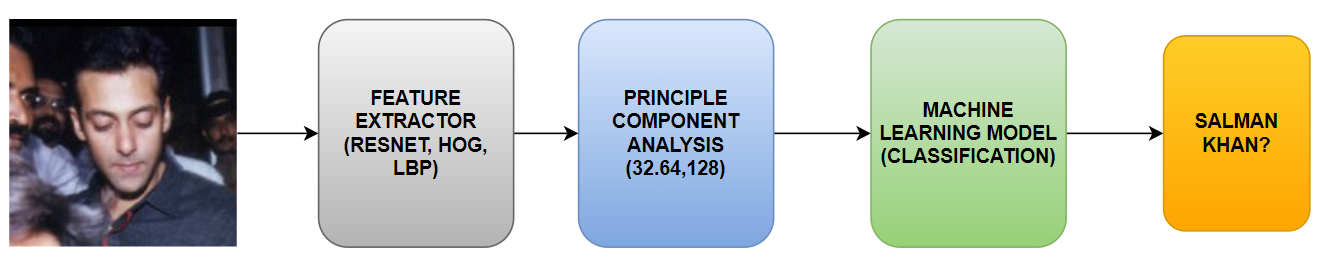
\includegraphics[width=1.0\textwidth]{Figs/lfw_image.png}
    \caption{Generalized working diagram}
    \label{fig:workflow}
\end{figure}

\begin{figure}[hbt!]
    \centering
    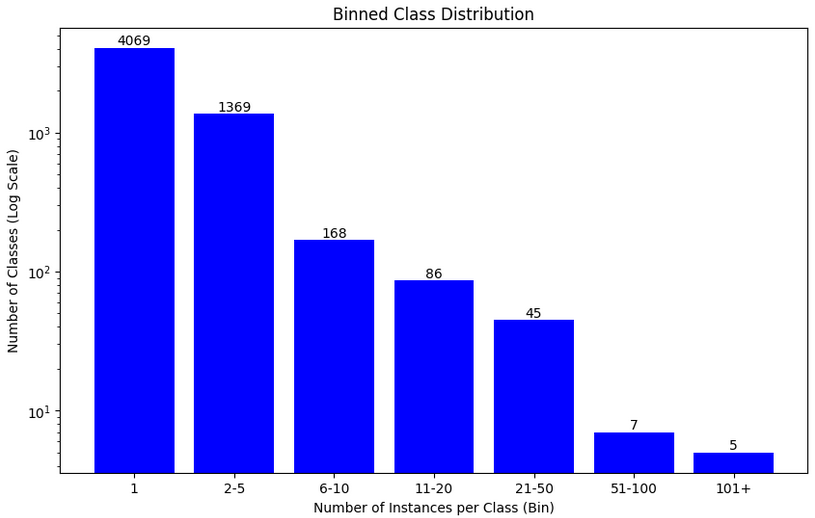
\includegraphics[width=0.8\textwidth,height=0.25\textheight]{Figs/Image.png}
    \caption{Class Imbalance}
    \label{fig:class_imbalance}
\end{figure}

	\newpage
	
	\section{Approaches Tried}
	
	In our study, we investigated several machine learning models to enhance facial recognition performance using the Labeled Faces in the Wild (LFW) dataset. Our objective was to determine the effectiveness of various feature extraction techniques and classification models.

\subsection*{Feature Extraction Methods}

We employed three distinct methods to extract features from the images:

\begin{enumerate}
    \item \textbf{Pre-trained ResNet Features\cite{resnet}:} Utilizing a pre-trained ResNet model, we extracted high-level features from the images, resulting in a 2048-dimensional feature vector per image. This approach leverages deep learning to capture intricate patterns and characteristics of faces.
    \item \textbf{Histogram of Oriented Gradients (HOG)\cite{hog}:} The HOG feature descriptor was used to capture edge and gradient structure information from the images, producing a 70,308-dimensional vector. This method is traditionally renowned for its effectiveness in object detection tasks.
    \item \textbf{Local Binary Patterns (LBP)\cite{lbp}:} We extracted texture features using the LBP technique, which provided a 256-dimensional feature vector per image. LBP is particularly useful for capturing fine-grained texture details that are often pivotal in facial recognition.
\end{enumerate}

\subsection*{Dimensionality Reduction with PCA}

Given the high dimensionality of the extracted features, especially from the ResNet and HOG methods, we applied Principal Component Analysis (PCA) \cite{PCA} to reduce the feature dimensions. This step was crucial to alleviate computational demands and to standardize the feature space across different methods for a fair comparison of model performances. PCA was tailored for each feature type, ensuring optimal dimension reduction while retaining significant variance in the data.

\subsection*{Classification Models}

We experimented with the following classification models on the dimensionally reduced features:

\begin{itemize}
    \item \textbf{K-Nearest Neighbors (KNN)\cite{knn}:} A simple yet effective model that classifies images based on the closest feature vectors in the training set.
    \item \textbf{Logistic Regression:} A fundamental statistical model used to estimate probabilities using a logistic function, ideal for binary classification tasks.
    \item \textbf{Support Vector Machine (SVM)\cite{svm}:} This model finds the hyperplane that best separates different classes in the feature space, which is critical in high-dimensional spaces.
    \item \textbf{Random Forest\cite{randomforest}:} An ensemble method that uses multiple decision trees to improve classification accuracy and control over-fitting.
    \item \textbf{XGBoost\cite{xgboost}:} An implementation of gradient boosted decision trees designed for speed and performance, which has proven effective in various machine learning competitions.
\end{itemize}

Each model was applied to the PCA-reduced features from the three extraction methods, and performance metrics were calculated to evaluate their efficacy in facial recognition tasks.We also experimented with the balanced version of Logistic Regression to address the significant class imbalance, but it incurred high computational costs without consistently improving the results. Consequently, we excluded it from the analysis table.
	\newpage

	
	\section{Experiments and Results}


\subsection*{Labeled Faces in the Wild (LFW) Dataset Overview}
The Labeled Faces in the Wild (LFW) \cite{Huang2012a} dataset is a key resource in computer vision, particularly valuable for the development and evaluation of face recognition technologies. The dataset comprises:
\begin{itemize}
    \item \textbf{Images:} Color photographs typically sized around 250x250 pixels, focusing on the face of individuals.
    \item \textbf{Number of Classes:} The dataset includes images of 5,749 different individuals, constituting a vast multi-class space.
    \item \textbf{Class Imbalance:} There is significant class imbalance, with some individuals represented by many images and others by very few.
\end{itemize}

This dataset poses substantial challenges such as high dimensionality of raw pixel data, the need for robust feature extraction to manage intra-class variation, and sophisticated machine learning techniques to address the significant class imbalance.

\subsection*{Experimental Setup and Model Parameterization}
\subsubsection*{Feature Extraction and Dimensionality Reduction}
To manage the high dimensionality of the face images and the expansive class space effectively, we applied the following feature extraction methods followed by Principal Component Analysis (PCA) to reduce dimensions:
\begin{itemize}
    \item Pre-trained ResNet Features
    \item Histogram of Oriented Gradients (HOG)
    \item Local Binary Patterns (LBP)
\end{itemize}

PCA was performed with dimensions of \textbf{32}, \textbf{64}, and \textbf{128} to find a balance between retaining essential features and reducing dimensionality for computational efficiency.

\subsubsection*{Classification Models and Parameters}
We utilized several classification models with specific configurations to efficiently process the data:
\begin{itemize}
    \item \textbf{K-Nearest Neighbors (KNN):} Configured with 5 neighbors to make the model sensitive enough to effectively capture the nuances between different faces, crucial given the high variability within the 5,749 classes.
    \item \textbf{Logistic Regression:} Using the `saga` solver, `L2` penalty, tolerance of 0.01, and up to 1000 iterations, these settings ensure the solver converges on a solution within a reasonable timeframe without sacrificing the accuracy needed to handle many classes.
    \item \textbf{SVM (LinearSVC):} Set with a regularization parameter \(C = 1\) and a maximum of 1000 iterations, optimizing for linear separability and managing the high dimensionality post-PCA reduction.
    \item \textbf{Random Forest:} 10 estimators, a max depth of 20, and `max features` set to `sqrt` to keep the model's complexity in check and prevent overfitting by considering a sufficient number of features at each split.
    \item \textbf{XGBoost:} 20 estimators and a max depth of 20, these settings offer a good trade-off between model complexity and learning ability, crucial in a dataset with a large number of classes.
\end{itemize}

Parameters not specifically mentioned were set to their default values in the scikit-learn library. This approach is designed to provide a thorough comparison across different feature extraction methods and model configurations, identifying the most effective techniques for facial recognition with the LFW dataset.

% \begin{table}[h!]
%     \centering
%     \caption{Performance of Classification Models on PCA-Reduced Features with Top-1 and Top-5 Accuracies and Execution Time}
%     \label{tab:performance_comparison}
%     \begin{adjustbox}{width=\textwidth,center}
%     \begin{tabular}{|c|c|c|c|c|c|}
%         \hline
%         \textbf{Feature Method} & \textbf{PCA Dimension} & \textbf{Model} & \textbf{Top-1 Accuracy} & \textbf{Top-5 Accuracy} & \textbf{Execution Time} \\
%         \hline
%         \multirow{15}*{ResNet} & \multirow{5}*{32} & KNN & 0.52 & 0.78 & - \\
%         \cline{3-6}
%         & & Logistic Regression & 1 & 1 & 1 \\
%         \cline{3-6}
%         & & SVM & - & - & - \\
%         \cline{3-6}
%         & & Random Forest & - & - & - \\
%         \cline{3-6}
%         & & XGBoost & - & - & - \\
%         \cline{2-6}
%         & \multirow{5}*{64} & KNN & - & - & - \\
%         \cline{3-6}
%         & & Logistic Regression & - & - & - \\
%         \cline{3-6}
%         & & SVM & - & - & - \\
%         \cline{3-6}
%         & & Random Forest & - & - & - \\
%         \cline{3-6}
%         & & XGBoost & - & - & - \\
%         \cline{2-6}
%         & \multirow{5}*{128} & KNN & - & - & - \\
%         \cline{3-6}
%         & & Logistic Regression & - & - & - \\
%         \cline{3-6}
%         & & SVM & - & - & - \\
%         \cline{3-6}
%         & & Random Forest & - & - & - \\
%         \cline{3-6}
%         & & XGBoost & - & - & - \\
%         \hline
%         \multirow{15}*{HOG} & \multirow{5}*{32} & KNN & - & - & - \\
%         \cline{3-6}
%         & & Logistic Regression & - & - & - \\
%         \cline{3-6}
%         & & SVM & - & - & - \\
%         \cline{3-6}
%         & & Random Forest & - & - & - \\
%         \cline{3-6}
%         & & XGBoost & - & - & - \\
%         \cline{2-6}
%         & \multirow{5}*{64} & KNN & - & - & - \\
%         \cline{3-6}
%         & & Logistic Regression & - & - & - \\
%         \cline{3-6}
%         & & SVM & - & - & - \\
%         \cline{3-6}
%         & & Random Forest & - & - & - \\
%         \cline{3-6}
%         & & XGBoost & - & - & - \\
%         \cline{2-6}
%         & \multirow{5}*{128} & KNN & - & - & - \\
%         \cline{3-6}
%         & & Logistic Regression & - & - & - \\
%         \cline{3-6}
%         & & SVM & - & - & - \\
%         \cline{3-6}
%         & & Random Forest & - & - & - \\
%         \cline{3-6}
%         & & XGBoost & - & - & - \\
%         \hline
%         \multirow{15}*{LBP} & \multirow{5}*{32} & KNN & - & - & - \\
%         \cline{3-6}
%         & & Logistic Regression & - & - & - \\
%         \cline{3-6}
%         & & SVM & - & - & - \\
%         \cline{3-6}
%         & & Random Forest & - & - & - \\
%         \cline{3-6}
%         & & XGBoost & - & - & - \\
%         \cline{2-6}
%         & \multirow{5}*{64} & KNN & - & - & - \\
%         \cline{3-6}
%         & & Logistic Regression & - & - & - \\
%         \cline{3-6}
%         & & SVM & - & - & - \\
%         \cline{3-6}
%         & & Random Forest & - & - & - \\
%         \cline{3-6}
%         & & XGBoost & - & - & - \\
%         \cline{2-6}
%         & \multirow{5}*{128} & KNN & - & - & - \\
%         \cline{3-6}
%         & & Logistic Regression & - & - & - \\
%         \cline{3-6}
%         & & SVM & - & - & - \\
%         \cline{3-6}
%         & & Random Forest & - & - & - \\
%         \cline{3-6}
%         & & XGBoost & - & - & - \\
%         \hline
%     \end{tabular}
%     \end{adjustbox}
% \end{table}
\begin{table}[h!]
    \centering
    \caption{Performance of Classification Models on PCA-Reduced Features with Top-1 and Top-5 Accuracies}
    \label{tab:performance_comparison}
    \begin{adjustbox}{width=\textwidth,center}
    \begin{tabular}{|c|c|c|c|c|}
        \hline
        \textbf{Feature Method} & \textbf{PCA Dimension} & \textbf{Model} & \textbf{Top-1 Accuracy} & \textbf{Top-5 Accuracy} \\
        \hline
        \multirow{15}*{ResNet} & \multirow{5}*{32} & KNN & 0.29 & 1.00 \\
        \cline{3-5}
        & & Logistic Regression & 0.52 & 0.78 \\
        \cline{3-5}
        & & SVM & 0.67 & 0.82 \\
        \cline{3-5}
        & & Random Forest & 0.63 & 0.76 \\
        \cline{3-5}
        & & XGBoost & 0.21 & 0.25 \\
        \cline{2-5}
        & \multirow{5}*{64} & KNN & 0.31 & 1.00 \\
        \cline{3-5}
        & & Logistic Regression & 0.70 & 0.89 \\
        \cline{3-5}
        & & SVM & 0.87 & 0.94 \\
        \cline{3-5}
        & & Random Forest & 0.55 & 0.68 \\
        \cline{3-5}
        & & XGBoost & 0.22 & 0.26 \\
        \cline{2-5}
        & \multirow{5}*{128} & KNN & 0.32 & 1.00 \\
        \cline{3-5}
        & & Logistic Regression & 0.73 & 0.91 \\
        \cline{3-5}
        & & SVM & 0.91 & 0.96 \\
        \cline{3-5}
        & & Random Forest & 0.36 & 0.51 \\
        \cline{3-5}
        & & XGBoost & 0.14 & 0.25 \\
        \hline
        \multirow{15}*{HOG} & \multirow{5}*{32} & KNN & 0.24 & 1.00 \\
        \cline{3-5}
        & & Logistic Regression & 0.57 & 0.76 \\
        \cline{3-5}
        & & SVM & 0.58 & 0.71 \\
        \cline{3-5}
        & & Random Forest & 0.42 & 0.53 \\
        \cline{3-5}
        & & XGBoost & 0.16 & 0,20 \\
        \cline{2-5}
        & \multirow{5}*{64} & KNN & 0.26 & 1,00 \\
        \cline{3-5}
        & & Logistic Regression & 0.83 & 0.93 \\
        \cline{3-5}
        & & SVM & 0.82 & 0.91 \\
        \cline{3-5}
        & & Random Forest & 0.39 & 0.49 \\
        \cline{3-5}
        & & XGBoost & 0.22 & 0.25 \\
        \cline{2-5}
        & \multirow{5}*{128} & KNN & 0.27 & 1.00 \\
        \cline{3-5}
        & & Logistic Regression & 0.97 & 0.99 \\
        \cline{3-5}
        & & SVM & 0.97 & 0.98 \\
        \cline{3-5}
        & & Random Forest & 0.37 & 0.46 \\
        \cline{3-5}
        & & XGBoost & 0.23 & 0.27 \\
        \hline
        \multirow{15}*{LBP} & \multirow{5}*{32} & KNN & 0.22 & 1.00 \\
        \cline{3-5}
        & & Logistic Regression & 0.03 & 0.09 \\
        \cline{3-5}
        & & SVM & 0.00 & 0.00 \\
        \cline{3-5}
        & & Random Forest & 0.39 & 0.51 \\
        \cline{3-5}
        & & XGBoost & 0.04 & 0.09 \\
        \cline{2-5}
        & \multirow{5}*{64} & KNN & 0.22 & 1.00 \\
        \cline{3-5}
        & & Logistic Regression & 0.03 & 0.09 \\
        \cline{3-5}
        & & SVM & 0.00 & 0.00 \\
        \cline{3-5}
        & & Random Forest & 0.33 & 0.43 \\
        \cline{3-5}
        & & XGBoost & 0.04 & 0.10 \\
        \cline{2-5}
        & \multirow{5}*{128} & KNN & 0.22 & 1.00 \\
        \cline{3-5}
        & & Logistic Regression & 0.03 & 0.09 \\
        \cline{3-5}
        & & SVM & 0.00 & 0.00 \\
        \cline{3-5}
        & & Random Forest & 0.15 & 0.24 \\
        \cline{3-5}
        & & XGBoost & 0.04 & 0.10 \\
        \hline
    \end{tabular}
    \end{adjustbox}
     \textbf{Note: All accuracies are computed using the entire dataset as training data.}
\end{table}
\subsection{ResNet Feature Extraction}
\begin{itemize}
    \item \textbf{Top-1 Accuracy:}
    \begin{itemize}
        \item SVM consistently outperformed other models across all PCA dimensions, achieving a peak accuracy of 91\% at 128 dimensions.
        \item Logistic Regression showed increasing accuracy with higher PCA dimensions, reaching up to 73\%.
        \item Random Forest performed well at lower dimensions but showed a significant drop at 128 dimensions (36\%).
        \item KNN and XGBoost were less effective, particularly XGBoost, which decreased significantly to 14\% at 128 dimensions.
    \end{itemize}
    \item \textbf{Top-5 Accuracy:}
    \begin{itemize}
        \item SVM led with up to 96\% at 128 dimensions, showing robust performance.
        \item Logistic Regression and KNN maintained high accuracy, with KNN consistently achieving 100\%.
    \end{itemize}
\end{itemize}

\subsection{Histogram of Oriented Gradients (HOG) Feature Extraction}
\begin{itemize}
    \item \textbf{Top-1 Accuracy:}
    \begin{itemize}
        \item Logistic Regression and SVM achieved nearly perfect performance at 128 dimensions with accuracies reaching 97\%.
        \item Random Forest and KNN showed lower performance, particularly at higher dimensions.
        \item XGBoost remained consistently low, peaking at 22\%.
    \end{itemize}
    \item \textbf{Top-5 Accuracy:}
    \begin{itemize}
        \item High performance for Logistic Regression and SVM, approaching 99\% at 128 dimensions.
    \end{itemize}
\end{itemize}

\subsection{Local Binary Patterns (LBP) Feature Extraction}
\begin{itemize}
    \item \textbf{Top-1 and Top-5 Accuracies:}
    \begin{itemize}
        \item Both Logistic Regression and SVM showed minimal effectiveness, with accuracies peaking only at 3\%.
        \item Random Forest had moderate success, highest at 39\% for Top-1 accuracy at 32 dimensions but declined with higher PCA settings.
        \item KNN and XGBoost demonstrated very low performance across all dimensions.
    \end{itemize}
\end{itemize}

\subsection{Discussion and Insights}
\begin{itemize}
    \item SVM and Logistic Regression generally provided the highest accuracies with ResNet and HOG features, whereas SVM's performance plummeted with LBP features. This suggests a need for feature extraction methods that better align with SVM’s capabilities. A notable observation not depicted in the analysis table is that despite its prolonged convergence time across all scenarios, SVM consistently delivered superior outcomes when paired with ResNet and HOG features.


\item One of the key challenges in the LFW dataset is the significant imbalance among classes, with some classes having many more samples than others. SVM's effectiveness in this context can be attributed to its margin optimization, which focuses on correctly classifying the most challenging examples near the decision boundary rather than merely optimizing overall accuracy. This characteristic allows SVM to perform well even when some classes are underrepresented.

    \item KNN showed excellent retrieval capabilities (Top-5 accuracy) but needs enhancements for precision in Top-1 rankings, possibly through method modifications or integrating different feature types. This discrepancy suggests that KNN can effectively retrieve groups of similar classes, but struggles with precisely identifying the most probable class. It indicates the model's sensitivity to the local structure of data where neighbors include the correct class but not as the closest match. This could be due to the vast and diverse class space where similar features may exist among different faces, thus confusing the model in precise ranking. Enhancing KNN's precision might require method modifications such as implementing distance weighting or incorporating additional or more discriminative feature types
    \item The choice of feature extraction methods and classifier combinations is critical in complex datasets, particularly those involving high dimensionality and class variability like facial recognition.
        \item The performance of XGBoost was consistently lower than other models, particularly in environments with high-dimensional data and large class spaces. This contradicts the expectations set by its gradient boosting capabilities, indicating that in this specific dataset, XGBoost may not effectively handle the complexity or the class imbalance as previously theorized.
     \item 
LBP features proved to be insufficiently discriminative for SVM classification, resulting in lengthy training times exceeding 14 hours and yielding low accuracy. This indicates the need for more complex or diverse features to improve model performance.
\end{itemize}


\subsection{Performance Metrics for SVM}

The Support Vector Machine (SVM) classifier demonstrated consistently high accuracy in our experiments, particularly when paired with robust feature extraction methods like ResNet and Histogram of Oriented Gradients (HOG). Below, we present the precision, recall, and F1-score for SVM in the context of these feature extraction techniques. These metrics are crucial for evaluating the effectiveness of the classifier in a multiclass setting.

\begin{table}[h]
\centering
\begin{tabular}{|c|c|c|c|}
\hline
\textbf{Feature Method} & \textbf{Precision} & \textbf{Recall} & \textbf{F1-Score} \\
\hline
ResNet & 0.96 & 0.98 & 0.97 \\
\hline
HOG & 0.99 & 1.00 & 1.00 \\
\hline
\end{tabular}
\caption{Precision, Recall, and F1-score for SVM using ResNet and HOG features.}
\label{tab:svm_metrics}
\end{table}

\textbf{Multiclass Formulation of Precision, Recall, and F1-Score}

In a multiclass classification context, precision, recall, and F1-score can be calculated for each class individually and then averaged to provide a global performance metric. The definitions are as follows:

\begin{itemize}
    \item \textbf{Precision} (Positive Predictive Value): The ratio of true positive predictions to the total predicted positives for a specific class.
    \item \textbf{Recall} (Sensitivity): The ratio of true positive predictions to the total actual positives for a specific class.
    \item \textbf{F1-Score}: The harmonic mean of precision and recall, providing a balance between the two. It is particularly useful when the class distribution is imbalanced.
\end{itemize}

Mathematically, for a specific class \( i \):

\begin{equation}
    \text{Precision}_i = \frac{TP_i}{TP_i + FP_i}
\end{equation}

\begin{equation}
    \text{Recall}_i = \frac{TP_i}{TP_i + FN_i}
\end{equation}

\begin{equation}
    \text{F1-Score}_i = 2 \cdot \frac{\text{Precision}_i \cdot \text{Recall}_i}{\text{Precision}_i + \text{Recall}_i}
\end{equation}

Where \( TP_i \) is the number of true positives, \( FP_i \) is the number of false positives, and \( FN_i \) is the number of false negatives for class \( i \).


	
	


% This report extensively explored the application of machine learning techniques to enhance facial recognition capabilities using the Labeled Faces in the Wild (LFW) dataset. A key aspect of this investigation was addressing the challenges posed by high dimensionality and class imbalance. Our findings suggest that certain models, particularly Support Vector Machines (SVM), demonstrated superior performance in managing these challenges effectively.

% \begin{itemize}
%     \item \textbf{High Class Space:} SVM, with its ability to construct an optimal hyperplane in high-dimensional spaces, excelled in environments with a vast number of classes. This model showed remarkable accuracy, especially in PCA-reduced spaces of 64 and 128 dimensions, achieving top-1 accuracies of 0.87 and 0.91, respectively.
%     \item \textbf{Class Imbalance:} Contrary to previous assessments, XGBoost did not perform as expected. It generally showed lower performance across all PCA dimensions, which suggests that its typical advantages in handling class imbalances were not realized in this dataset.
% \end{itemize}

% % The study confirmed that a strategic combination of feature extraction, dimensionality reduction, and careful selection of classifiers is essential for optimizing facial recognition systems. The utilization of advanced models like SVM and XGBoost can significantly enhance the reliability and accuracy of facial recognition technologies in real-world scenarios dominated by complex data characteristics.
% The study confirms the necessity of carefully selecting feature extraction methods and classifier combinations. While advanced models like SVM showed potential, XGBoost did not meet the expectations set by its theoretical capabilities in this scenario.



% Overall, this research contributes valuable insights into the development of more sophisticated and effective facial recognition systems, paving the way for future advancements in the field.
\section{Summary}

This report investigates the application of advanced machine learning techniques to enhance facial recognition capabilities using the \textit{Labeled Faces in the Wild} (LFW) dataset. We address the inherent challenges of high dimensionality and class imbalance through innovative feature extraction methods and dimensionality reduction techniques. Specifically, we utilize Pre-trained ResNet, Histogram of Oriented Gradients (HOG), and Local Binary Patterns (LBP) for feature extraction, followed by Principal Component Analysis (PCA) to achieve a balance between data representativeness and computational efficiency.

Our findings reveal significant insights into the performance trade-offs among various feature-classifier combinations, which are crucial for optimizing both accuracy and computational resources in real-world scenarios. The study highlights configurations that effectively enhance the performance of facial recognition systems. For example, the SVM classifier consistently outperforms other models when paired with ResNet and HOG features across different PCA dimensions, demonstrating high accuracy and robustness. Conversely, the performance of XGBoost is notably lower, suggesting that it may not handle the complexities and class imbalance of the dataset effectively.

The report contributes to the field by outlining effective strategies for managing large-scale, imbalanced datasets in facial recognition technologies. It provides a comprehensive analysis of how different combinations of feature extraction methods and classifiers can be optimized to improve the accuracy and reliability of facial recognition systems.

	



	\bibliography{refs}
	
	\appendix
	
	\section{Contribution of each member}
	\label{sec:contribution}
	\begin{enumerate}
	\item Anuj Rajan Lalla: Implemented models and maintained GitHub repo structure. Prepared Report, Github Code and Spotlight video
	\item Sarth Sanjay Joshi: Midreport preparation , contribution in GitHub code. Web deployment of best model and web demo
 \item Abhinav Swami: Preparation of Accuracies code. Preparation of project page using HTML and CSS . 
	\item Satyam Sharma: Midreport preparation and code . Feature Extraction and references for report
 \item Sanjeet Athawale: Midreport preparation and code , Feature extraction code and accuracies code

	
	\end{enumerate}
    	
	
\end{document}